
\section{Motivation}

As a software engineers,
we often came across software distributed
in a form of docker containers alongside
of traditional binary files,
articles comparing Docker to the other kind of virtualization techniques
and DevOps research papers comparing the performance of cloud instances in AWS,
but did not know what it was about.
The main goal of this research is to provide an answer
for an important question, whether it is worth
to change our infrastructures
from virtualized hardware to Docker, or stick to KVM, for example.

Virtualization was invented long before the mid-2000s,
but has only became mainstream for the industry at this time.
Smart virtualization engines such as Linux-based QEMU, KVM, Xen
and their Windows-based rival Hyper-V changed the IT industry forever,
sufficiently decreasing the need for dedicated and local hardware.

This shift has turned a cloud computing from abstract theory to the reality,
creating large profits for cloud providers like Amazon AWS,
Microsoft Azure and Google.
However, the virtualization was not perfect, as any advanced technology:
as obvious as their advantages were, it had many
drawbacks as we will discuss in section 2.6.

With the first release of its state-of-the-art Docker library for Linux,
developer Solomon Hikes provided its own way of solving these problems,
which has not only became a successful startup
with capitalization of over one hundred eighty millions
USD\footnote{United States Dollars} as of June 2016\cite{DockerCapitalization}.
It also became a major breakthrough in the IT Field, almost pushing the existing
businesses and startups in maintaining advanced virtualized infrastructure
to the edge of survival or even completely eliminating
them from the market for good\cite{DockerImpact}.

\section{Long way to Docker}

Some technologies evolved themselves from the existing ideas
or approaches at the time of invention, and Docker is no exception.
The aim of this section is to provide an overview of the main competitive
technologies referenced as industry standardards
before the era of Docker, their advantages and disadvantages.

\subsection{Server architecture without virtualization}

A traditional server is just a hardware unit
which has an operating system installed,
and then supervises applications running.
It can be seen in the Figure \ref{fig:TraditionalAndVirtualInfra},
where it becomes clear that only a single
operating system can be executed over the hardware at every single moment of time.
This operating system is then responsible for providing multi-user access and
application control.

\begin{figure}
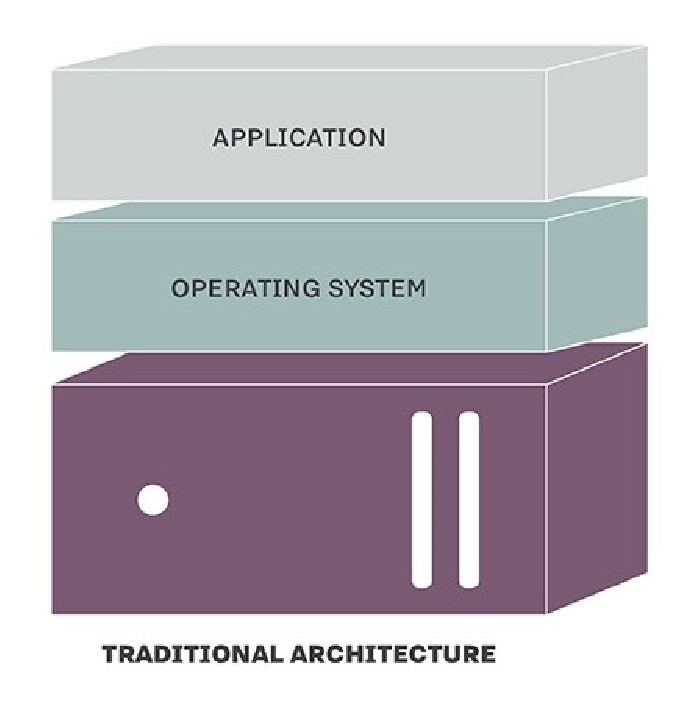
\includegraphics[height=3in, width=3in]{traditional}
\caption{Principal scheme of Data center architecture without virtualization}
\cite{TraditionalAndVirtualInfra}
\label{fig:TraditionalAndVirtualInfra}
\end{figure}

Though perfectly well suitable for normal users, this architecture
has proven itself as unreliable, non-scalable,
and generally not suitable for long-term enterprise environments support.
The operating system layer was usually installed manually or with
installation scripts specially written for that purpose,
and the enterprise application running inside these
environments were configured from within the OS by the system administrators.

\subsection{Virtualization definition and explanation}

\begin{definition}
Virtualization is a technology of technology that enables sharing of
existing hardware resources amongst the "host" operating system,
which has a direct access to the hardware resources and where the
virtualization program is started, and some of the "guest" operating systems,
which lifecycle is maintained and supervised by the abovementioned software.
\end{definition}

As can be seen in the Figure \ref{fig:TraditionalAndVirtualInfra1},
the virtualization layer is responsible for interacting with the hardware
(It can be a Virtual Machine Monitor or a Host OS)
Therefore, multiple operating systems can be started on top of that layer.
These OS are then responsible for application supervision.

With the invention of the virtualization,
it has become possible for one server to
offer its users multiple operating systems at a time
significantly decreasing stall times and the need for excessive hardware.
Moreover, it became possible to sell the unused
server power to the other commercial entities or private customers,
bringing additional revenue to the organization.

\subsection{Binary virtualization}

Binary translation is translation of code from one
instruction set to another. There are basically two types of binary translation-
static binary translation, where the translation is achieved by
converting all the source code to target
architecture without running the code, and
dynamic binary translation, where the translation is achieved during the runtime.

This approach is used in many modern
virtualization engines like VMWare and Valgrind\cite{SWVirtPrez}.

\begin{figure}
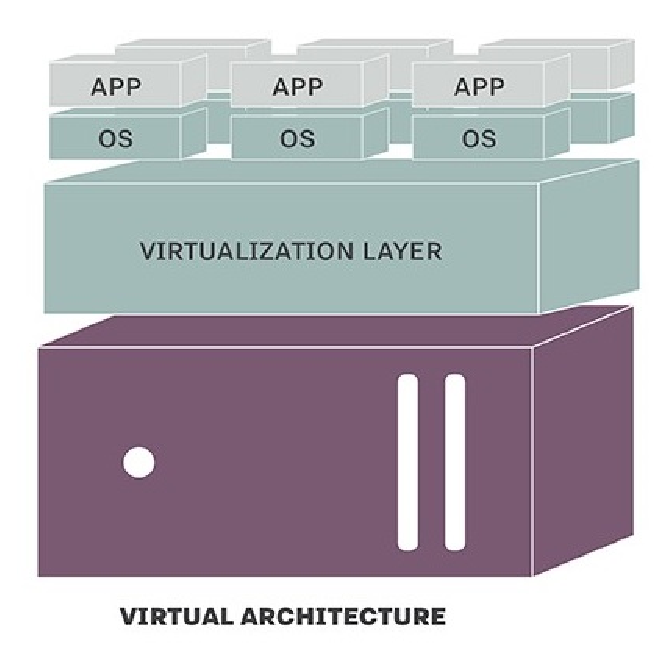
\includegraphics[height=3in, width=3in]{virtualized}
\caption{Principal scheme of virtualized infrastructure}
\cite{TraditionalAndVirtualInfra1}
\label{fig:TraditionalAndVirtualInfra1}
\end{figure}

\subsection{Paravirtualization}

First implemented and desciribed by Xen Project,

\begin{definition}
Paravirtualization (PV) is a virtualization technique
introduced by the Xen Project team, later adopted by other
virtualization solutions. PV does not require virtualization extensions from
the host CPU and thus enables virtualization on hardware architectures that do
not support Hardware-assisted virtualization.
However, PV guests and control domains require kernel
support and drivers that required special kernel builds in the past,
but are now part of the Linux kernel as well as other
operating systems\cite{ParavirtualizationDefinition}.
\end{definition}

It is clearly shown in the Figure \ref{fig:ParavirtualizationPic}:
Xen Backend provides its own core components, and the VM0 (or Dom0)
kernel communicates
with Hardware using that layer. The VM0 also provides
its communication backend for the other virtual system (Guest OS)
\begin{figure}
\includegraphics[height=3in, width=3in]{paravirtualized}
\caption{Principal scheme of paravirtualization initially made by Xen project}
\cite{ParavirtualizationPic}
\label{fig:ParavirtualizationPic}
\end{figure}

\subsection{Hardware-assisted virtualization}

With growing demand of personal customers
and commercial entities for enhancing VM performance
CPU manufacturers introduced
their new virtualization technologies - Intel VT and AMD-V.
A set of new instructions and, what is more important, a new privilege level
was added as well.
In the traditional x86 architecture,
operating system kernels expect direct CPU access
to the Ring 0, which is the most privileged level.
With software virtualization, guest operating
systems cannot run in Ring 0 because
the VMM\footnote{Virtual Machine Monitor} is being executed there.
The guest operating systems must therefore run in Ring 1,
but because some of the instructions must still be executed in Ring 0,
it must have been paravirtualized which resulted
in significant performance decrease\cite{HWAssistedVirt}.

With Intel VT and AMD-V, a hypervisor can then run at a "Ring -1";
so the guest operating systems can run in the Ring 0.
There is no need for paravirtualization,
the VMM does less work, and
the performance hit is therefore significantly reduced.

\subsection{Unsolved problems of the virtualization}

Virtualization technologies have many advantages as discussed before.
However, some issues could not be addressed by these technologies:
\begin{enumerate}
\item \textit{Scalability}

It is hard to add VM to the clusters,
set them up or remove in case
of need.

\item \textit{Maintenance}

Virtual systems need to be updated and backed up regularly to
prevent the loss of important business information.
With VMs, the updates need to be performed inside of Guest OS,
what is inconvenient or, in case of the necessary virtualization layer update,
all of the virtualized infrastructure must be stopped in order to do that.

\item \textit{Additional staff and reeducation}
With the complexity of the infrastructures
growing exponentially, the need for additional
employments and reeducation of existing employees
made an impact on the industry\cite{VirtualizationProblems}.
\end{enumerate}

\section{Docker principles}

In 2010, individual developer Solomon Hikes came up with an idea that was
supposed to provide an answer to all of the challenges brought up by different
virtualization techniques: instead of virtualizing hardware resources running
several operating systems at the same time, it would have been possible
to launch only one instance of an OS image and spare not only storage and memory capacity,
but also a CPU operations by performing all
OS activities (like rescheduling) only once, which should theoretically
improve performance
The goal of this chapter is to provide detailed overview of Docker architecture
and the ways it does perform its tasks.

\subsection{Container}

As stated by the Docker Inc., the inventor of Docker technology,

\begin{definition}
An image is a lightweight, stand-alone,
executable package of a piece of software that includes everything
needed to run it: code, runtime,
system tools, system libraries, settings\cite{DockerDefinition}.
\end{definition}

Container is another type of virtualization approach.
Containers and virtual machines have
similar resource isolation and allocation benefits,
but function differently because containers
virtualize the operating system instead of hardware.
Containers are believed to be more portable and
efficient,as stated in
the official Docker blog\cite{DockerEfficiency}.

The relationship of an image with
a container is like that of a program and a process -
just like a process is an incarnation of a program
the container is an incarnation of an image.

An example of a container can be
seen in the Figure \ref{fig:DockerContainerPic}.
In this figure, there can clearly be seen a Java Enterprise Edition application
running on Debian inside a container and PHP with MySQL running
on Ubuntu in another container and so on.
It is also shown, that they are sharing
one and the same Kernel avoiding redundancy in using it
over and over again like in VM\footnote{Virtual Machine}.

\begin{figure}
\includegraphics[height=3in, width=3in]{dockerContainer}
\caption{Some examples of Docker containers}
\cite{DockerContainerPic}
\label{fig:DockerContainerPic}
\end{figure}

\subsection{Microarchitecture}

Docker is a software product consisting mainly of a
library written in Go programming language
which acts as an intermediary between apps packaged
in the container and the Linux kernel.

Exactly like paravirtualization, at the time of its market show up
it required special builds of linux kernel, which provided the Docker core with
functionality later. After its broad adoption by the industry, these features
were included in all standard linux kernel builds.

Because of that, most of the current Docker function can now be simulated
using these advanced features without installation of additional components.

As can be seen in the Figure \ref{fig:DockerArch}, the Docker consists
of continous process dockerd, which then supervises other
components using REST\footnote{Representational state transfer}
and gets messages back from them. Docker has its
own CLI\footnote{Console Line Interface} which can be used by the local
user, but there is even more than that:
usage of REST as one of the most influencial currently implemented
standards in the Web gives many advantages to the Docker core making it possible
not only to connect several engines into connecting networks,
but also to provide reliable communication between several containers running on
one image, as it is described later\cite{DockerArch}.

\begin{figure}
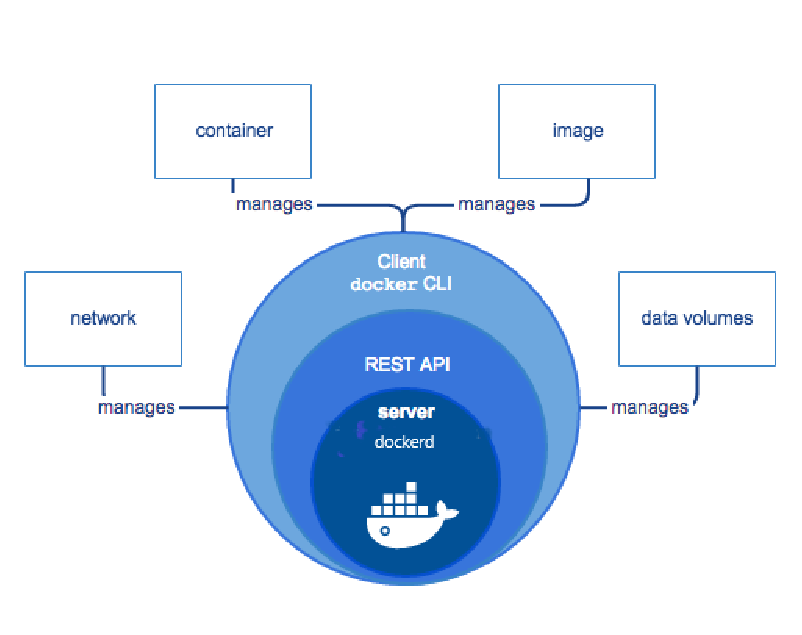
\includegraphics[height=3in, width=3in]{dockerarch}
\caption{Scheme of Docker architecture}
\cite{DockerArch}
\label{fig:DockerArch}
\end{figure}

Without the following advanced Linux kernel features,
the development of Docker would not have been possible
(shown in Figure \ref{fig:DockerLinuxKernelPic}):

\begin{figure}
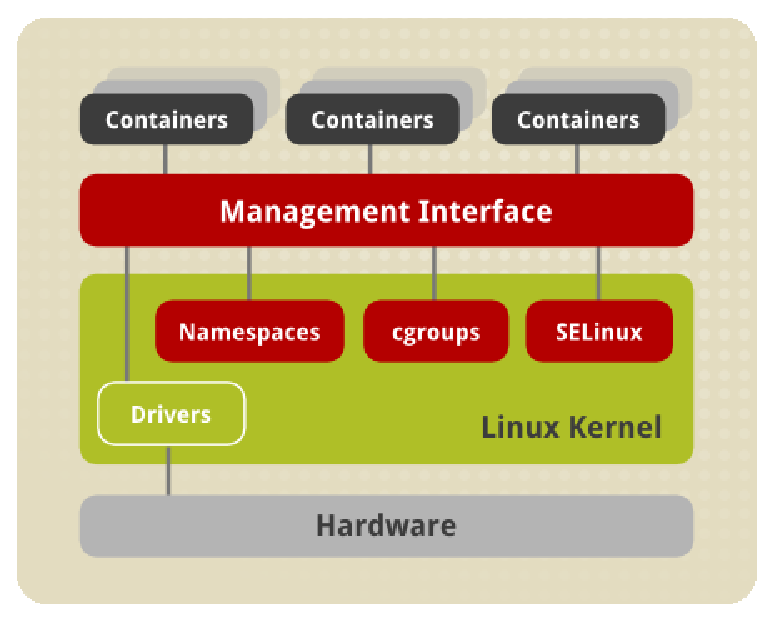
\includegraphics[height=3in, width=3in]{dockerLinuxKernel}
\caption{Linux kernel features Docker containers take use of}
\cite{DockerLinuxKernelPic}
\label{fig:DockerLinuxKernelPic}
\end{figure}

This figure shows the most important features
of linux kernel used by Docker engine. The meaning and
functions of these figures are described right here:

\begin{enumerate}
\item \textbf{control groups} (named \textbf{cgroups} for the sake of simplicity) is
a feature developed by Google
for AOSP\footnote{Android open source project} and merged
into the Linux kernel version 2.6.24\cite{CGroupsMerged}
which allows the kernel to restrict
each application to the specific set of resources or allocate them -
such as CPU time, system memory, network bandwidth,
or combinations of these resources - among user-defined groups
of tasks (processes) running on a system\cite{CGroupsDefinition}.

An example of such resources division is
shown on Figure \ref{fig:DockerCGroupsPic}.
As can be derived there, it is possible to assign
particular resources
like CPU\footnote{Central Processing Unit} and Memory to the
processes needing it the most -
in this case we reserve 2 CPUs and one RAM
unit to a web server and 4 CPUs and two RAM modules
to the MySQL database respectively.

\begin{figure}
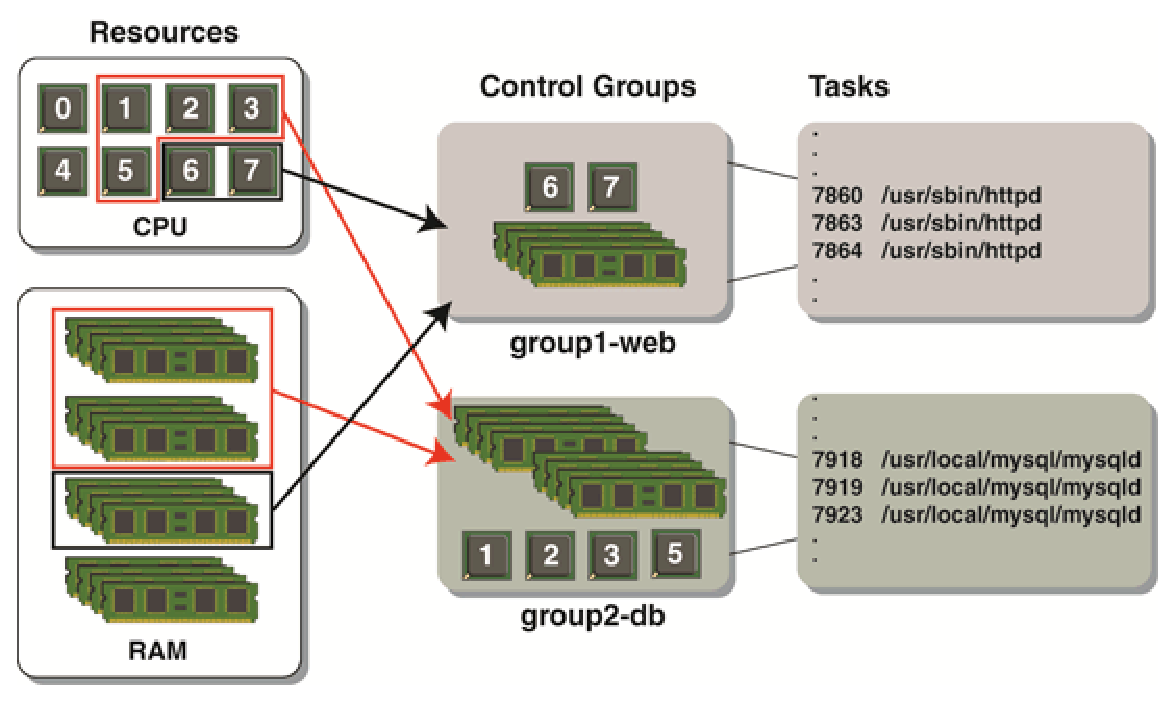
\includegraphics[height=3in, width=3in]{dockerCGroups}
\caption{Example of dividing resources between Docker containers using cgroups}
\cite{DockerCGroupsPic}
\label{fig:DockerCGroupsPic}
\end{figure}

\item \textbf{SELinux} - a special kernel extension, which adds advanced security features to
the OS, mainly fine-grained file control, but can also be applied
for the interprocess communication and network resources\cite{SELinuxDef}.

SELinux plain architecture description is
described on the Figure \ref{fig:DockerSELinuxPic} -
after each action request there is a query to the SELinux policy
database performed by SELinux security server. If positive, the
resource previously asked for is returned to the request maker. If negative,
there is a denial message passed back.

\begin{figure}
\includegraphics[height=3in, width=3in]{seLinux}
\caption{SELinux architecture}
\cite{DockerSELinuxPic}
\label{fig:DockerSELinuxPic}
\end{figure}

This is one of the kernel features, which has utter importance for Docker,
because without it would not have been possible to isolate files or ports
of the containers from the other containers trying to access this files,
which in turn would have led to security issues.
Docker employees have even described their software as being "Secure by Default"
in their blog post \cite{SELinuxDockBlog} because of an advantageous
usage of this technology

\item \textbf{namespaces} - a feature that is essential
to the functioning of containers.
For example, the PID\footnote{Process Identifier} namespace
is what keeps processes
in one container from seeing or interacting with processes
in another container (or, for that matter, on the host system).
A process might have the apparent PID 1 inside a container,
but if examined it from the host system,
it would have an ordinary PID
The PID namespace is the mechanism for remapping PIDs
inside the container. Likewise,
there are other namespaces (e.g. net, mnt, ipc, uts)
that (along with cgroups) provide
the isolated environments known as containers\cite{DockerNamespaces}.
The user namespace, then, is the mechanism
for remapping UIDs inside a container, and this is the newest
namespace to be implemented
in the Docker Engine,
starting in the version 1.10\cite{DockerSuccessNamespaces}.

\item \textbf{netlink} - provides a convenient way of communication
between userspace and the Linux kernel space.
Communication is made by means of casual sockets,
but using a special protocol which is called the AF\_NETLINK\cite{NetlinkOverview}.

It allows one to interact with large portions of kernel subsystems
like routing, iptables, various interfaces, net packets filter.
Not only that, it is made possible to communicate directly with a kernel
module of one own implementation, provided that
there are implemented means of handling that messages.

Each netlink message implements a header,
defined as nlmsghdr structure,
and also contains some bytes of useful load also called as a payload.
This payload can be some kind of structure, too, or it can carry raw data
Message, which can be partitioned during delivery process.
In that case each next package of a sequence has a flag NLM\_F\_MULTI,
and the last one is sealed with the NLMSG\_DONE flag.
For the purpose of message parsing, there is an entire macro set
defined in the header files rtnetlink.h and netlink.h\cite{NetlinkPacket}.

Docker has a pure implementation of netlink
in Go language that is open source for the community extensions
and usage in private projects.
This package can be used to create interfaces,
bridges, set IP address and other settings on network interfaces,
move network interfaces into different linux namespaces,
and so on.
This is the same code that handles creating the pairs and assigning
an IP Address to each of the containers created in Docker.

\item \textbf{AppArmor} - Linux security module
that protects an operating system and its applications from security threats.

The main advantage of it is simplicity when comparing to SELinux.
It works by applying special profiles to the container processes,
but cannot even come close
to the granularity SELinux provides\cite{AdrMouAppArmor:2016}.

To use it, a system administrator associates an
AppArmor security profile with each program.
Docker expects to find an AppArmor policy loaded and enforced.

Docker automatically generates and loads a default profile for containers
named docker-default. On Docker versions 1.13.0 and later, the Docker
binary generates this profile in tmpfs and then loads it into the kernel.
On Docker versions earlier than 1.13.0, this
profile is generated in /etc/apparmor.d/docker instead.

These feature is applied on containers, not the dockerd.

This feature may be turned off by passing a special
key when deploying a container.

\item \textbf{capabilities} - Dockers core component, dockerd,
requires root privileges at the time for correct work.
However, if Docker developers made a mechanism of waiving this requirement on
some types of containers, turning Linux binary (normal user or root) permissions
approach into more than hundred different settings allowing containers
to perform some operations without root permission for more security inside
a container\cite{AdrMouCapabilities:2016}.

\end{enumerate}

Moreover, the docker library is able to determine when multiple container
applications share the same libraries
and provide it for them at the time needed\cite{AdrMouContainersBinaries:2016}.
The main advantage of Docker is that it uses already existing features
provided by the Linux operating system.

\subsection{Docker Image}

To run a container, a docker image must be created.
An image is compiled by docker engine itself,
using a script provided by user called Dockerfile.
One of the most powerful features of Docker is inheritance,
so usual approach in the industry
is to pull a base image - an existing image
where custom configuration can be added. Default settings will be
reused and extended it with
new features later when there is
such a necessity\cite{AdrMouImagesBasics:2016}.

This is shown in the Figure \ref{fig:DockerFilePic}:
after a Dockerfile is written, it is compiled to an image by the Docker Engine
and can now be deployed as a container and stopped later.
The image itself can be pushed to the registry, in this
particular case to DockerHub or pulled from there.

\begin{figure}
\includegraphics[height=3in, width=3in]{dockerFile}
\caption{Dockerfile, image and registry relationships}
\cite{DockerFilePic}
\label{fig:DockerFilePic}
\end{figure}

\subsection{Using a container}

Once an image is created, it can be deployed into a container. A
container in terms of docker is nothing more than a running
instance of Host OS, where the docker is installed. It can be placed
in the cloud or on the local hardware.
Created containers can be launched, stopped, and queried for their
current state for maintenance work at will, exactly like normal virtual
machine can be. Upon container creation it is possible to pass
different launch parametres like an automatic restart if the server
has been turned off by some reason\cite{AdrMouContainerUsage:2016}.

\subsection{Union file system}

While proven to reduce average CPU load and memory usage by
eliminating the redundant duplication of the OS components of the
virtual environments,
unionfs (Union File System, further referred as UFS), a file system
is one of the most crucial parts of docker system.
In terms of Docker UFS it is called "Storage Driver"\cite{AdrMouUFS:2016}
UFS consits of "layers", abstract file system units clearly separated
from each other, with some of them write-protected. This allows
docker core to maintain one and the only copy of the operating
system files necessary for its working declaring it unchangeable
while keeping the changeable files belonging to different images
unreachable from within other layers thus making it impossible to
alter or delete them, drastically improving the security of the virtual
environments.

There are several underlying file systems that
implement UFS and can be chosen as a storage
driver in Docker\cite{AdrMouUFS:2016}:
\begin{enumerate}
\item AUFS
\item Overlay
\item BTRFS
\item ZFS
\item Device Mapper
\item VFS
\end{enumerate}

Adrian Mouat advises all Docker users in his book
to choose AUFS or Overlay as storage
driver even despite the need
to apply kernel updates\cite{AdrMouUFSAdvise:2016}

\subsection{Container registry}

As stated before in the section 3.1, docker image consists of multiple layers.
It is supposed to be convenient for the end user,
but has a fundamental problem: if we have
n images based on some kind of operating system, and we need
to distribute it to m servers, the OS image itself will be downloaded
n x m times, which leads to increased
load on the docker CDN \footnote{Content delivery network}

But Docker engineers have found a way to solve this problem by providing
a special service called Docker registry. It is a special service for uploading
custom images or its updates in a way, that only the necessary layers will be
downloaded by the consumers\cite{AdrMouRegistries:2016}.

Docker Registry is provided by Docker Inc. and is available
as a free public service or open-source software
for the installation on the own infrastructure.
That way the commercial entities, developer teams or even individuals having a
wish to hide their images from the public access,
are not bound to the usage of Docker Inc. as their unique provider. That means
no vendor lock-in is present\cite{AdrMouRegistries:2016}.

\subsection{Container interaction}

Because of an architecture and restrictions of Docker, it is only possible for
one layer to pass messages to an another layer by using ports opened for them.
In case when there is more than one container
instance running on the Docker server, it can become increasingly difficult for
to users to maintain them. And that is what
orchestration, described in section 4, is for.

\subsection{Docker on Windows}

Docker support is integrated into a wide range of development tools
from Microsoft, into operating systems and cloud infrastructure, including
the following technologies:
\begin{enumerate}
\item Windows Server 2016
\item Hyper-V
\item Visual Studio
\item Microsoft Azure
\end{enumerate}

Embedded support of Docker containers was added in Windows Server 2016 and it
is offered  two ways of  deploying them: Windows Server Containers and
Hyper-V Containers, which provides additional level of
isolation for multi-tenancy environments\cite{DockerOnWindows}.

In Windows, everything is arranged a bit differently in comparison to Linux.
The architecture of most high-level components looks exactly like Linux.
Here one can find the same Remote API, the same working tools.
However, Windows and Linux kernels are far different.
Microsoft is applying a slightly different approach to the design of the
kernel than the one developed by the Linux community.
Namely, the term "kernel mode" in Microsoft language refers not only to the
core of the system, but also to the level of hardware abstractions, and to
various system services.
There are modules for managing objects, processes, memory, security,
cache, PnP technology, power, settings, I/O operations.
All together, this is called the Windows executive system.

Kernel features in Windows do not have namespaces and control groups.
Instead, the Microsoft team, working on the new version of Windows Server 2016,
introduced the
so-called "Compute Service Layer"\cite{DockerOnWindowsMicrosoftBlog},
an additional layer of services at the operating
system level that provides namespace functions, resource management,
and features similar to UFS.
There is nothing on the Windows platform that corresponds
to the dockerd and its environment.
Instead, CSL provides public interface to the container
and is responsible for managing the containers, performing operations
such as launching and stopping them, but it does not control their status.
It replaces the dockerd and
abstracts the low-level capabilities that kernel provides.

\subsection{Performance of a container against VM}

On July 21, 2014 IBM released its research paper
on performance comparison between KVM and Docker
and got the following conclusions as a result of an
extensive test they made\cite{IBMResearchPaperOnPerformance}:

\begin{enumerate}
\item \textit{Docker equals or
exceeds KVM\footnote{Kernel-Based virtual machine}
performance in every case they tested.}
\item \textit{Both forms of virtualization have drawbacks
when it comes to tasks with
extensive I/O\footnote{Input/Output} load}
\item \textit{KVM is less suitable for workloads that are latency-sensitive
or have high I/O rates.}
\item \textit{Docker's NAT\footnote{Network Address Translation}
has big overhead
for workloads with high packet rates.}
\item \textit{Containers can also eliminate the distinction between
IaaS\footnote{Infrastructure-as-a-Service paradigm}
and "bare metal" non-virtualized servers since
they offer the control and isolation of VMs
with the performance of bare metal.}
\end{enumerate}

\section{Orchestration}

\begin{definition}
Orchestration is a process of setting up, controlling, updating
and performing maintenance works of complex applications containing more than
one container on appropriate hosts. An orchestration system may also include support for scaling,
automatic failover, and node rebalancing\cite{AdrMouOrchestration:2016}.
\end{definition}

Contrary to the virtualized environments, where this
process is complicated and can only be automated using advanced (and mostly
proprietary) software products, Docker offers tools for its users and customers
which are stated to make these processes simple and convenient:

\subsection{Docker Machine}

With Docker Machine, one can install the Docker engine on virtualized
hosts and manage them. A "Machine" is used to create Docker
hosts on local Operation System (Mac or Windows box), on a
network, in a data center, or even on cloud Providers.
One can start, stop, inspect and restart a managed host
with the docker-machine commands, upgrade the Docker client/daemon, and
even configure a Docker client to talk to your host. There are different
benefits with Docker Machine. With Docker Machine, one can provision
multiple remote Docker hosts on various flavours of Linux.
Additionally, it is possible to run Docker on older Mac or Windows systems.
Basically, Docker Machine is a tool for provisioning and
managing hosts with Docker Engine on them\cite{DockerMachine}.
Docker Machine is mainly used for two broad use cases.

If one works primarily on an older Mac or Windows that
does not meet the requirements for the new Docker apps,
Docker Machine is needed in order to "run Docker" locally.
If one wants to provision Docker hosts on remote systems and wants to have
an efficient way to provision multiple Docker hosts on a network,
in the cloud or locally, Docker Machine is needed.
Independently form the used Operating System, one can install
Docker Machine on it and use the provisioned commands to manage
large numbers of Docker hosts\cite{MTBAHeise}.
It automatically creates hosts,
installs Docker Engine on them and eventually
configures the docker clients, as shown schematically on the
Figure \ref{fig:DockerMachinePic}.
This picture depicts schematically that provisioning of Docker hosts can be done
on local machine, in the cloud or on a virtual machine belonging
to a data center. In the end, each managed
host(Machine) is the combination of a Docker host and a configured client.

\begin{figure}
\includegraphics[height=3in, width=3in]{dockerMachine}
\caption{Docker Machine scheme}
\cite{DockerMachinePic}
\label{fig:DockerMachinePic}
\end{figure}

\subsection{Docker Compose}

Docker Compose is a Docker service which can start,
stop or hold on complex docker infrastructures
containing more than one container with exposed port
just like if it were a normal application\cite{DockerCompose}.

Some examples of such applications
can be LAMP\footnote{Linux Apache MySQL PHP} Stack
or JEE\footnote{Java Enterprise Edition} Framework
implementations like EAS\footnote{Enterprise Application Server}
Glassfish, WildFly or Mojarra, as these software
complexes use multi-tier architecture, where a database server is
started separately from the enterprise application server,
but should be used and maintained as a single application.

Docker compose requires special configuration file called
docker-compose.yml shown on Figure \ref{fig:DockerComposeFilePic}
for the environment setup
as well as the Dockerfiles of all of the
containers to configure them according to the users
preferences defined in these files previously\cite{DockerCompose}.

\begin{figure}
\includegraphics[height=3in, width=3in]{dockerComposeExample}
\caption{Example of Docker Compose configuration file}
\cite{DockerComposeFilePic}
\label{fig:DockerComposeFilePic}
\end{figure}

As stated in the Docker documentation, Compose is particularly suitable
for development environments,
automated test enviroments and continous integration

\subsection{Docker Swarm}

Basically, Docker Swarm is a clustering tool for Docker Containers.
Docker Swarm enables Users a straight forward opportunity,
to merge multiple Docker hosts into a cluster\cite{DockerSwarmDefinition}.
The behaviour of swarm is the same as a dockerd.
Clustering is an important feature of container technologies,
because it creates a cooperative group of systems.
With that, one can provide redundancy.
A Docker Swarm cluster also provides the
ability to add or remove the number of instances of a given container
image as computing demands change
as can be seen in the Figure \ref{fig:DockerSwarmPic}:
A Swarm consist of a manager (also called Master) and
as many slaves (also called workers) as wanted.
The Swarm-Manager is responsible for the scheduling
of containers on all slaves and is the primary
interface to access on the resources of the cluster\cite{DockerSwarmKeyConcepts}.
With Swarm one can achieve greater performance and
better usability of resources, since it uses
scheduling capabilities to ensure sufficient resources for
the containers inside the cluster. This technology ensures that containers
are launched/run on systems with adequate resources, while maintaining
necessary performance levels\cite{DockerSwarmHowNodesWork}.

\begin{figure}
\includegraphics[height=3in, width=3in]{dockerSwarm}
\caption{Docker Swarm architecture}
\cite{DockerSwarmPic}
\label{fig:DockerSwarmPic}
\end{figure}

\subsection{Kubernetes support}

It is worth mentioning,
that Docker will start
supporting its main rival in the orchestration field, Kubernetes,
which is much more popular amongst clients and developers as Docker Swarm,
in its Enterprise Edition subscription since 17 October 2017,
as it is explained in Docker Blog entry\cite{DockerKubernetesSupport}.

The overview of this orchestration tool, its advantages and disadvantages
and the comparison with Docker Swarm, is, however, not a part of
this research paper.

\section{Conclusions}

As a result of this research work, it became clear to us that, first of all,
the approach of container virtualization or containerization
is the future of software deployment, because it not only reduces complexity of
different types of infrastructure like content delivery network,
but also reduces server load,
increases security of the deployed application,
because the possibly infected software cannot
escape its file system layer and has no direct access
to the operating system where the docker process is running, and is
especially usable for shipping software
images to the different types of customers,
from the most inexperienced ones to hardcore professionals.

When it comes to performance, based on the section 3.9, it exceeds
that of a virtual machine,
even taking a performance
hit of container isolation problematics into account.
Of course, the Docker approach has drawbacks, too, mainly
because it is relatively new to the market,
and it is pretty hard for industry to find
a sufficient amount of system administrators or special
administering software qualified to support advanced docker infrastructures,
but we are pretty sure that this technology does belong to the
present and the future of software development and deployment.

\appendix
%Appendix A
\section{Contents}
\subsection{Motivation}
\subsection{Long way to Docker}
\subsubsection{Server architecture without virtualization}
\subsubsection{Virtualization definition and explanation}
\subsubsection{Binary virtualization}
\subsubsection{Paravirtualization}
\subsubsection{Hardware-assisted virtualization}
\subsubsection{Unsolved problems of the virtualization}
\subsection{Docker architecture}
\subsubsection{Container}
\subsubsection{Microarchitecture}
\subsubsection{Docker Image}
\subsubsection{Using a container}
\subsubsection{Union File System}
\subsubsection{Container registry}
\subsubsection{Container interaction}
\subsubsection{Docker on Windows}
\subsubsection{Performance of a container against VM}
\subsection{Orchestration}
\subsubsection{Docker Machine}
\subsubsection{Docker Compose}
\subsubsection{Docker Swarm}
\subsubsection{Kubernetes support}
\subsection{Conclusions}
\subsection{References}
